\documentclass[11pt]{amsart}
\usepackage{geometry}
\geometry{letterpaper}
%\geometry{landscape}                % Activate for for rotated page geometry
%\usepackage[parfill]{parskip}
% Activate to begin paragraphs with an empty line rather than an indent
\usepackage{graphicx}
\usepackage{amssymb}
\usepackage{epstopdf}
\usepackage{booktabs}
\usepackage{siunitx} % international system units, for tabs to align at dot

\DeclareGraphicsRule{.tif}{png}{.png}{`convert #1 `dirname #1`/`basename #1 .tif`.png}

\title{\Large ToFu's benchmarking\\
  \small AWP18-EEG-CEA-Mendoza}

\author{Laura S. Mendoza}
\author{Didier Vezinet}

\date{}                           % Activate to display a given date or no date

\begin{document}
\maketitle

\section{Starting Point}

ToFu's versioning is set automatically with each \verb|git| tag.
We will set as a reference point the version number \verb|1.3.22-6-g45cb446|,
which also corresponds to the \verb|git| tag.

\subsection{Geometry definitions}
\label{sect:configs}
In order to have an extensive benchmarking, we need to set a series of tests
configurations that will encompass the maximum scenarios, as well as allow us
to test the speed-up of simple yet essential methods. Let us first define the
different geometries:\\

\begin{itemize}
	\item Tests with only a vessel:
	\begin{itemize}
		\item  Config A1:
		\begin{itemize}
			\item  WEST -- V1 (realistic) : 63 points
		\end{itemize}
		\item  Config A2:
		\begin{itemize}
			\item  TER -- Test (artificial) : 551 points
		\end{itemize}
		\item  Config A3:
		\begin{itemize}
		\item  WESTSep -- Test (artificial, inspired by the
                  separatrix of an experimental shock of WEST) : 1001 points\\
		\end{itemize}
	\end{itemize}
	\item    Tests with a vessel and structural elements:
	\begin{itemize}
		\item  Config B1: 'min' (only axisymmetric structures)
		\begin{itemize}
			\item  Ves: WEST V0
			\item  Struct:
			\begin{itemize}
				\item      Baffle : Baffle-V0
				\item      Upper divertor : UpDiv-V1
				\item      Lower divertor : LowDiv-V1
			\end{itemize}
		\end{itemize}
	      \item  Config B2: 'light'  (same as B1 + some toroidal
                structures)
		\begin{itemize}
			\item  Ves: WEST V0
			\item  Struct:
			\begin{itemize}
				\item      Baffle: Baffle-V1
				\item      Upper divertor: UpDiv-V2
				\item      Lower divertor: LowDiv-V2
				\item      Inner Bumpers: InnerBumpers-V1
				\item      Outer Bumper: OuterBumper-V1
				\item      IC antennas: IC1-V1 + IC2-V1
                                  + IC3-V1
			\end{itemize}
		\end{itemize}
	      \item  Config B3: 'full'
                \begin{itemize}
			\item  Ves: WEST-V0
			\item  Struct:
			\begin{itemize}
			        \item      Baffle: Baffle-V2
			        \item      Upper divertor: UpDiv-V3
			        \item      Lower divertor: LowDiv-V3
			        \item      Inner Bumpers: InnerBumpers-V3
				\item      Outer Bumper: OuterBumper-V3
				\item      IC antennas: IC1-V1 + IC2-V1
                                  + IC3-V1
				\item      LH antennas : LH-V1, LH2-V1
				\item      Ripple : Ripple-V1
				\item      VDE : VDE-V0
			\end{itemize}
	\end{itemize}
\end{itemize}
\end{itemize}

\begin{figure}[h]
  \caption{Examples of geometry configurations: A2 and A3}
  \centering
  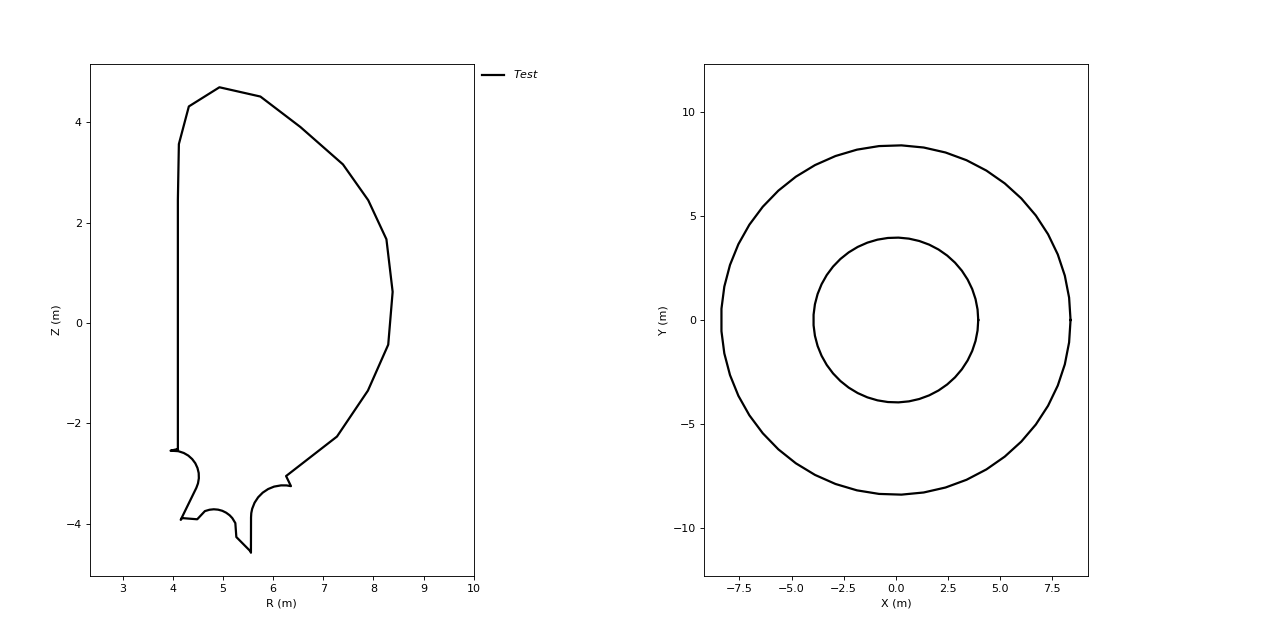
\includegraphics[width=0.5\textwidth]{./figures/figure.png}
  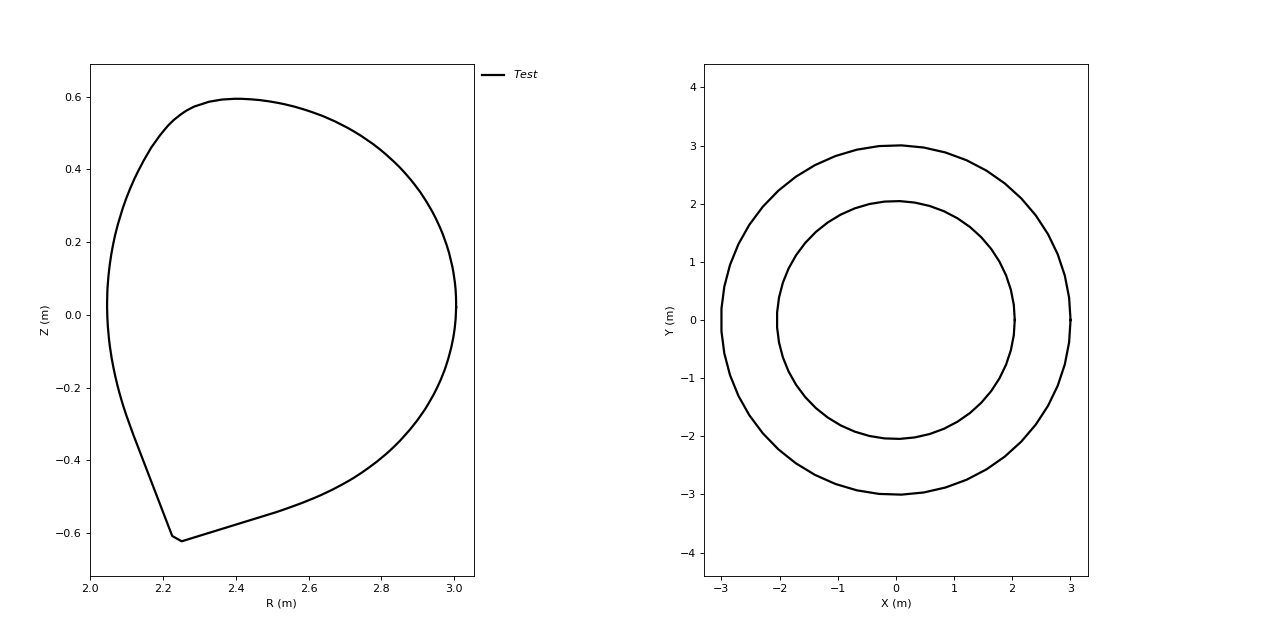
\includegraphics[width=0.5\textwidth]{./figures/figure2.png}
\end{figure}



The camera is defined as following.
The point of convergence in $(X,Y,Z)$ coordinates is $P = [1.5,3.2,0.]$ it is pointed towards the
device with direction $\vec{n}_{In} = [-0.5,-1.,0.]$ (normalized) of magnitude $F = 0.1$. The
camera is dicretized in a set of LOS, which have a director vector of $D_{12} = [0.3,0.1]$.
We will vary the number of lines of sights in a camera, $N_i = 10^i$, with $i=0, \cdots, 6$.\\

\section{Set of tests and initial times}

As a baseline, we use the set of ToFu's unit-tests for the geometry part. There are a total of 13
tests testing the most low-level functions, we will exclude for this part the 13th.
The table \ref{tab:UT} shows the execution time needed
for each test on different machines.

\begin{table}[h] % just use this specifier if really needed.
    \centering
    \caption{Execution time of unit tests 1 to 13, time computed as the mean of 5 runs}\label{tab:UT}
	%    \begin{tabular}{@{}lrrrrrr@{}} 
	\sisetup{round-mode=places}
     \begin{tabular}{@{}l*{6}{S[table-format=1.2e-1,scientific-notation=true]}@{}}    
    \toprule
      \textbf{Machine} & {Test 1} & {Test 2} & {Test 3} & {Test 4} & {Test 5} & {Test 6} \\ \midrule
      Ubuntu & 0.0003126 & 0.0004468 & 0.0001554 & 0.0003012 & 0.000482 & 0.0052582  \\
      Sirrah & 0.0086206 & 0.0003952 & 0.0001658 & 0.00032  &  0.0005792 & 0.0081134\\
      Atlas & 0.0 & 0.0 & 0.0 & 0.0 & 0.0 & 0.0 \\
      \bottomrule
    \end{tabular}\\
    %\begin{tabular}{@{}lrrrrrr@{}} 
\begin{tabular}{@{}l*{6}{S[table-format=1.2e-1,scientific-notation=true]}@{}}      
    \toprule
      %% \textbf{Machine} & Test 7 & Test 8 & Test 9 & Test 10 & Test 11 & Test 12 & Test 13 \\ \midrule
      %% Ubuntu  & 0.0476964 & 0.005901 & 0.0350598 & 0.0479324 & 0.1106498 & 0.0283896 & 0.0061352 \\
      %% Sirrah &   0.0516274  & 0.006856 &  0.046948  &  0.05907 &   0.132117 &  0.036295 &   0.0066378\\
      %% Atlas &  0.0 & 0.0 &  0.0 & 0.0 & 0.0 & 0.0 & 0.0 \\
      \textbf{Machine} & {Test 7} & {Test 8} & {Test 9} & {Test 10} & {Test 11} & {Test 12}  \\ \midrule
      Ubuntu  & 0.0476964 & 0.005901 & 0.0350598 & 0.0479324 & 0.1106498 & 0.0283896  \\
      Sirrah &   0.0516274  & 0.006856 &  0.046948  &  0.05907 &   0.132117 &  0.036295 \\
      Atlas &  0.0 & 0.0 &  0.0 & 0.0 & 0.0 & 0.0 \\
      \bottomrule
    \end{tabular}
\end{table}

In addition we tested the different combination of geometries configurations with the camera defined in
Section~\ref{sect:configs} and the different number of LOS, on the method from the \verb|geometry| module,
\verb|LOS_Calc_PInOut_VesStruct|. This method will be the focus of our optimization. The inital times
are summed up in table ADDTABLEREF.


\begin{table}[h] % just use this specifier if really needed.
    \centering
    \caption{Execution time of the method on different configurations on  Sirrah }
    \label{tab:LOS_init_sirrah}
    % Visionner le code LaTeX du paragraphe 0
	\sisetup{round-mode=places}
     \begin{tabular}{@{}c*{6}{S[table-format=1.2e-1,scientific-notation=true]}@{}}
       \toprule
       \multicolumn{1}{c}{config} & {A1} & {A2} & {A3} & {B1} & {B2} & {B3}\\
       \midrule
       V$1$      & 0.0002830028533935 & 0.000288724899291 & 0.0002665519714355 & 0.00046873092651 & 0.001762390136718 & 0.10256910324096\\
       V$10$     & 0.0002257823944091 & 0.000367641448974 & 0.0004203319549560 & 0.00061988830566 & 0.004924774169921 & 0.36218905448913\\
       V$10^2$   & 0.0004072189331054 & 0.001023530960083 & 0.0014843940734863 & 0.00082159042358 & 0.034385681152343 & 2.87086915969848\\
       V$10^3$   & 0.0019013881683349 & 0.008644580841064 & 0.0144457817077636 & 0.00331640243530 & 0.327978849411010 & 28.4926774501800\\
       V$10^{4}$ & 0.0145549774169921 & 0.083053588867187 & 0.1412739753723144 & 0.02720856666564 & 3.225792169570923 & 282.840265989303\\
       V$10^{5}$ & 0.1442494392395019 & 0.837333202362060 & 1.3932499885559082 & 0.26165747642517 & 33.53607034683227 & 2845.76993727684\\
       V$10^{6}$ & 1.5589430332183838 & 8.447954416275024 & 13.903767108917236 & 2.77517032623291 & 329.3016924858093 & 29030.8106548786\\
       \bottomrule
     \end{tabular}
\end{table}




\begin{table}[h] % just use this specifier if really needed.
    \centering
    \caption{Execution time of the method on different configurations on Ubuntu}
    \label{tab:LOS_init_sirrah}
    % Visionner le code LaTeX du paragraphe 0
	\sisetup{round-mode=places}
     \begin{tabular}{@{}c*{6}{S[table-format=1.2e-1,scientific-notation=true]}@{}}
       \toprule
       \multicolumn{1}{c}{config} & {A1} & {A2} & {A3} & {B1} & {B2} & {B3}\\
       \midrule
       V$1$      & 0.00028395652770996094 & 0.00022459030151367188 & 0.00025248527526 & 0.000370264053344 & 0.00156831741333 & 0.11810493469238281\\
       V$10$     & 0.00027346611022949220 & 0.00028276443481445310 & 0.00033211708068 & 0.000433683395385 & 0.00490784645080 & 0.41411495208740234\\
       V$10^2$   & 0.00055027008056640620 & 0.00079059600830078120 & 0.00115370750427 & 0.000623226165771 & 0.02871012687683 & 3.511296510696411\\
       V$10^3$   & 0.00200867652893066400 & 0.00719046592712402340 & 0.01251053810119 & 0.003671884536743 & 0.26398158073425 & 32.56944823265076\\
       V$10^{4}$ & 0.01538681983947753900 & 0.06923341751098633000 & 0.11263871192932 & 0.023092269897460 & 2.56951785087585 & 310.23827385902405\\
       V$10^{5}$ & 0.11928200721740723000 & 0.67663884162902830000 & 1.12707686424255 & 0.207307100296020 & 25.8998832702636 & 3202.3827385902405\\
       V$10^{6}$ & 1.16081881523132320000 & 6.79208517074585000000 & 11.3137621879577 & 2.094620227813720 & 258.980541706085 & 31723.827385902405\\
       \bottomrule
     \end{tabular}
\end{table}




\begin{table}[h] % just use this specifier if really needed.
    \centering
    \caption{Execution time of the method on different configurations on  Sirrah }
    \label{tab:LOS_init_sirrah}
    % Visionner le code LaTeX du paragraphe 0
	\sisetup{round-mode=places}
     \begin{tabular}{@{}l*{4}{S[table-format=1.2e-1,scientific-notation=true]}@{}}
       \toprule
       \textbf{Number of LOS} &  {$10^3$} & {$10^4$} & {$10^5$} & {$10^6$}\\
       \midrule
       original       & 32.569 & 310.23 & 3202.38 & 31723.827 $(~8$h$48)$\\
       optimized   & 0.0258 & 0.2720 & 2.73581 & 26.589564 $(<30$s$)$\\
       parallelized (32 threads) & 0.0136 & 0.0466 & 0.3640 & 2.9188 \\
       \bottomrule
     \end{tabular}
\end{table}

\end{document}
